\chapter{Risk as Runway: Putting It All on the Line}

This School of Hard Knocks interview, curated for the Entrepreneurship course by LazyingArt LLC, gives us a compact case study in entrepreneurial risk. The speaker does not begin with a theory. He begins with a newborn on the way, roughly the last \(\$1{,}000\) in a family bank account, a decision to quit and write a first product, the sale of a motorcycle, and finally a partner who contributes personal money. The mathematical structure is therefore deliberately modest: cash becomes time, assets become runway, and risk becomes visible as the distance between a commitment and the resources available to sustain it.

\section{The Question: Risk Before Theory}

The opening question asks for the biggest risk the speaker ever took and how important risk has been to him. That order matters. We are not first handed a definition of risk; we are asked to listen for it inside a sequence of decisions.

The speaker's first response is conversational: this is a story. That cue tells us how to read the passage. The lesson is not a slogan about boldness. It is a small balance-sheet narrative in which family obligations, product-building time, and scarce capital are introduced one by one.

For these notes, we will use the word \emph{risk} in a narrow working sense: a commitment has been made, the outcome is uncertain, and the available resources may not be enough to reach the next viable state. In this interview the next viable state is not described by revenue, valuation, or exit. It is simply enough time to keep building the first product until another source of support appears.

\section{The Constraint: Newborn, Cash, and No Cushion}

The first concrete quantity is the remaining cash balance. The speaker says he had a newborn on the way and had gotten down to probably the last \(\$1{,}000\) in his bank account or his wife's bank account. We should keep the approximation visible, because the transcript itself is approximate.

\begin{equation}
C_0 \approx \$1{,}000 .
\end{equation}

Here \(C_0\) denotes the initial cash balance at the moment the story becomes acute. It is not a formal accounting statement. It is the number the speaker uses to make the risk concrete.

A small amount of cash is not automatically a crisis. It becomes a crisis when it is compared with the rate at which time consumes money. If \(B\) denotes monthly burn, then a standard runway model would write

\begin{equation}
R_0 \approx \frac{C_0}{B},
\end{equation}

where \(R_0\) is runway measured in months. The transcript does not give \(B\), so we do not compute \(R_0\). The formula is useful only because it names the pressure: with a newborn coming and only about \(\$1{,}000\) left, the problem is no longer just money. It is time.

\section{The Decision Point}

The next move is the risky one. The speaker decides to quit and start writing his first product. The order is important: the product is not a decorative detail added after the decision. It is the reason the decision can be analyzed as entrepreneurial risk rather than mere withdrawal from employment.

In a product venture, cash is not only a reserve. It is the material that buys uninterrupted work. A month of survival can become a month of writing, testing, selling, or finding help. That does not make the choice safe, but it explains why the speaker narrates it as a business risk rather than only a personal hardship.

\subsection{Question \& Answer}

\paragraph{Question.}
Was quitting with a newborn on the way and roughly the last \(\$1{,}000\) in the family bank account calculated risk or recklessness?

\paragraph{Answer.}
The transcript does not give enough information to settle that as a general judgment. What it does show is the mechanism by which the speaker tried to keep the risk alive long enough to become productive. He did not describe a large cash reserve or a known investor. He described a first product, an asset that could be sold, and later a partner who brought in personal money. The risk was extreme, but it was not narrated as empty bravado. It was narrated as a sequence of runway extensions.

\section{Converting an Asset into Time}

After the decision to quit and build, the speaker says he sold the one asset he had at the time: a motorcycle. That sale got them through another month or two. This is the central mathematical move of the interview. An asset is converted into time.

Let \(A_{\mathrm{moto}}\) denote the proceeds from the motorcycle sale. The cash update is

\begin{equation}
C_1 = C_0 + A_{\mathrm{moto}} .
\end{equation}

If the monthly burn rate is \(B\), then the additional runway created by the motorcycle sale is

\begin{equation}
\Delta R_{\mathrm{moto}} \approx \frac{A_{\mathrm{moto}}}{B}.
\end{equation}

The speaker supplies the duration, not the sale price. He says the sale got them through another month or two. In cautious notation,

\begin{equation}
\Delta R_{\mathrm{moto}} \approx 1\text{ to }2 \text{ months}.
\end{equation}

This should not be inverted into a motorcycle valuation. We do not know \(B\), and we do not know \(A_{\mathrm{moto}}\). The useful point is the structure of the move: a non-cash asset becomes a temporary extension of product-building time.

\paragraph{A worked runway update.}
The transcript supports the following schematic calculation, with no hidden numerical assumptions:

\begin{align}
C_0 &\approx \$1{,}000, \\
C_1 &= C_0 + A_{\mathrm{moto}}, \\
R_1 &\approx \frac{C_1}{B}
     = \frac{C_0 + A_{\mathrm{moto}}}{B}, \\
R_1 - R_0 &\approx \frac{A_{\mathrm{moto}}}{B}
          \approx 1\text{ to }2 \text{ months}.
\end{align}

This is the whole derivation. We begin with scarce cash, add the proceeds of the motorcycle sale, and express the result as added runway. The calculation is not meant to make the risk look tidy. It is meant to preserve the speaker's practical logic: the sale bought time.

\section{Partner Capital and Shared Exposure}

The next transition is from solitary exposure to shared exposure. The transcript is slightly garbled at this point, but the reliable content is clear enough: a future business partner came on board and put in some of his personal money. The sequence now has a second capital event.

Let \(K_{\mathrm{partner}}\) denote the partner's personal contribution. Then the schematic cash state becomes

\begin{equation}
C_2 = C_1 + K_{\mathrm{partner}}
    = C_0 + A_{\mathrm{moto}} + K_{\mathrm{partner}} .
\end{equation}

The corresponding runway expression is

\begin{equation}
R_2 \approx \frac{C_0 + A_{\mathrm{moto}} + K_{\mathrm{partner}}}{B}.
\end{equation}

Again, the numbers are not available. We do not know the contribution, the burn rate, the equity arrangement, the product timeline, or the eventual company economics. But the narrative logic is precise. First there is the household cash constraint. Then the founder converts a personal asset into another month or two. Then a partner contributes personal money. The risk remains real, but it is no longer carried in exactly the same way.

\section{The Sequence as a Runway Diagram}

The following diagram is a transcript-derived reconstruction, not a screenshot or board copy. It keeps the sequence narrow and vertical so that the structure survives a small page format.

\begin{figure}
\centering
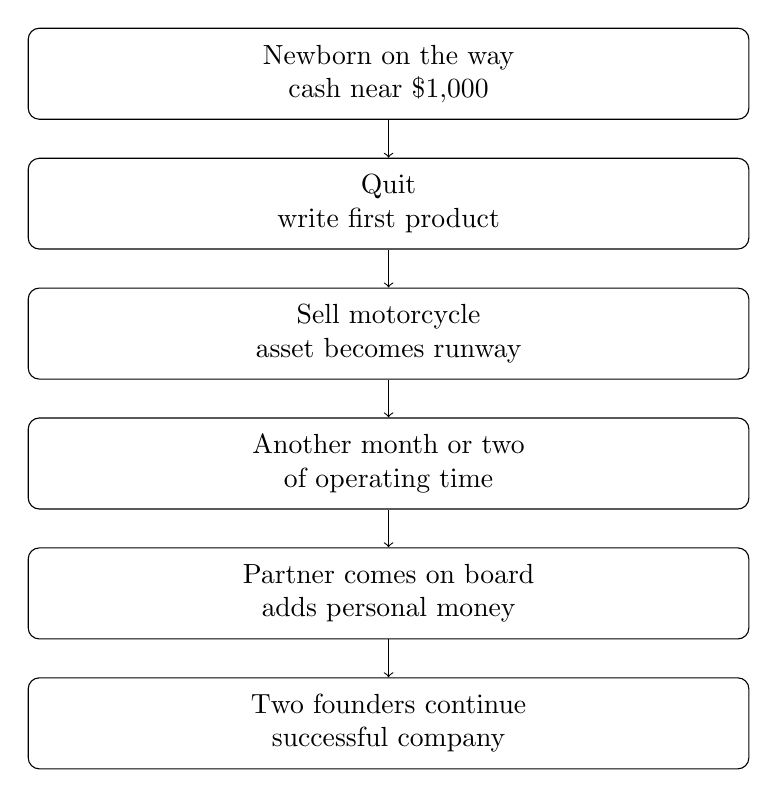
\begin{tikzpicture}[x=1cm,y=1cm]
\node[draw, rounded corners, align=center, text width=0.72\linewidth, inner sep=6pt] (a) at (0,0)
{Newborn on the way\\cash near \(\$1{,}000\)};

\node[draw, rounded corners, align=center, text width=0.72\linewidth, inner sep=6pt] (b) at (0,-1.65)
{Quit\\write first product};

\node[draw, rounded corners, align=center, text width=0.72\linewidth, inner sep=6pt] (c) at (0,-3.30)
{Sell motorcycle\\asset becomes runway};

\node[draw, rounded corners, align=center, text width=0.72\linewidth, inner sep=6pt] (d) at (0,-4.95)
{Another month or two\\of operating time};

\node[draw, rounded corners, align=center, text width=0.72\linewidth, inner sep=6pt] (e) at (0,-6.60)
{Partner comes on board\\adds personal money};

\node[draw, rounded corners, align=center, text width=0.72\linewidth, inner sep=6pt] (f) at (0,-8.25)
{Two founders continue\\successful company};

\draw[->] (a) -- (b);
\draw[->] (b) -- (c);
\draw[->] (c) -- (d);
\draw[->] (d) -- (e);
\draw[->] (e) -- (f);
\end{tikzpicture}
\caption{A transcript-derived runway sequence: cash constraint, product work, asset liquidation, partner capital, and eventual company success.}
\end{figure}

The diagram also shows why the final sentence has force. The speaker's claim that he put it all on the line is not merely emotional emphasis. It is the retrospective summary of a chain in which nearly all available resources were committed before the outcome was secure.

\section{Putting It All on the Line}

The final claim is that saying he put it all on the line is not an understatement. We should be careful with this conclusion. The company later became successful, but the later success does not retroactively make the original risk easy. The point of the story is the opposite: the risk is meaningful because the outcome was not already guaranteed.

The business mechanism can be summarized as a sequence of capital states:

\begin{align}
C_0 &\approx \$1{,}000, \\
C_1 &= C_0 + A_{\mathrm{moto}}, \\
C_2 &= C_1 + K_{\mathrm{partner}}.
\end{align}

Each update corresponds to a spoken beat in the interview. The first is the family cash constraint. The second is the motorcycle sale. The third is the partner's personal contribution. If we preserve that order, we preserve the commercial reasoning of the story.

\section{Summary}

This chapter's mathematical payload is small but sharp. Risk is treated as runway under pressure. The speaker begins with a newborn on the way and roughly the last \(\$1{,}000\), chooses to quit and write a first product, sells the one asset he names, gains another month or two, and then survives long enough for a partner to contribute personal money.

We should not add a theory that the interview does not provide. There is no visible board work, no probability model, no valuation, and no equity calculation. What the transcript gives us is a disciplined sequence: scarce cash, product commitment, asset liquidation, partner capital, and retrospective recognition that the founder really did put everything on the line.